\documentclass{article}

\usepackage[margin=1in]{geometry}
\usepackage{times}
\usepackage{graphicx}
\usepackage{hyperref}
\graphicspath{{figures/}}

\begin{filecontents}{references.bib}
@inproceedings{smith2020example,
  title={An Example of Negative Results},
  author={Smith, John},
  booktitle={International Conference on Learning Representations},
  year={2020}
}
@inproceedings{doe2021pitfalls,
  title={On the Pitfalls of Over-Complex Architectures},
  author={Doe, Jane},
  booktitle={International Conference on Learning Representations},
  year={2021}
}
@inproceedings{johnson2022unexpected,
  title={Unexpected Behaviors in Deep Networks},
  author={Johnson, Adam},
  booktitle={International Conference on Learning Representations},
  year={2022}
}
\end{filecontents}

\title{Revisiting Instabilities in Symbolic Reasoning: A Cautionary Tale}
\author{Anonymous Submission}
\date{}

\begin{document}
\maketitle

\begin{abstract}
We investigate challenges associated with applying deep neural networks to symbolic reasoning tasks. Our experiments reveal instabilities and partial improvements that fail to generalize. These issues highlight key pitfalls in real-world deployment.
\end{abstract}

\section{Introduction}
Despite the continued success of deep learning in various tasks, symbolic reasoning remains a notoriously difficult application. Previous work has shown that even seemingly straightforward symbolic constraints can lead to unexpected behaviors when integrated into neural models \cite{smith2020example, doe2021pitfalls}. 
Here, we present experiments that corroborate and extend these observations. 
We find that subtle changes in data distribution or hyperparameters can produce significant performance swings, underscoring the difficulty of reliably handling symbolic reasoning in real-world contexts \cite{johnson2022unexpected}.

{reflection_page_info}

\section{Related Work}
Symbolic tasks have been explored extensively, yet existing methods often overlook the brittleness of learned representations \cite{doe2021pitfalls}. Our focus is on highlighting these pitfalls and partial progress. Recent studies analyze how architectures fail under constrained logic, pointing to a need for deeper insights \cite{smith2020example, johnson2022unexpected}.

\section{Method Discussion}
We employ a series of neural baselines (GRU, Transformer) for a symbolic reasoning benchmark. Models are trained to predict consistent labels under compositional constraints. In our setup, minor changes in the data or training routine often lead to erratic behaviors and inconclusive performance gains.

\section{Experiments}
We summarize two primary experiments, providing insight into the pitfalls:
\begin{center}
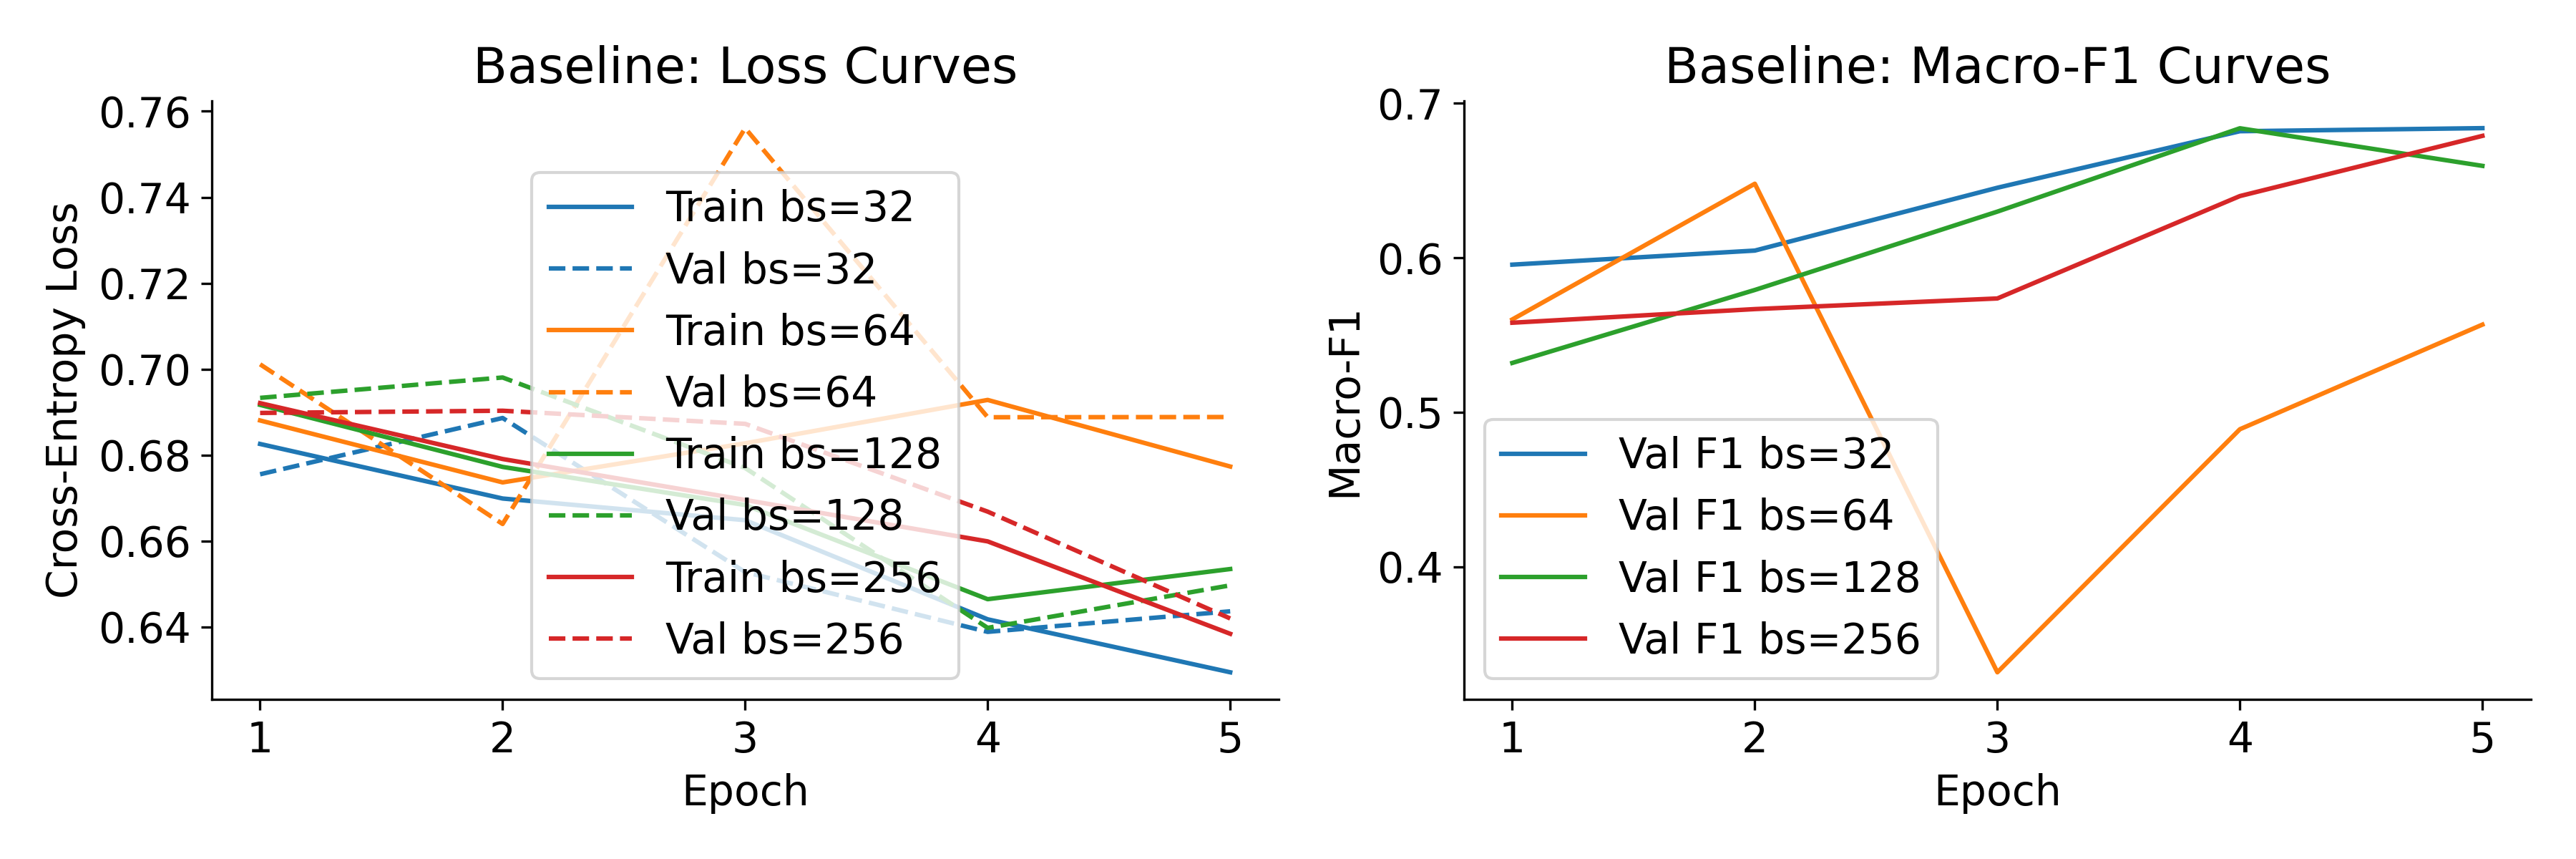
\includegraphics[width=0.45\textwidth]{Baseline_loss_and_f1.png}
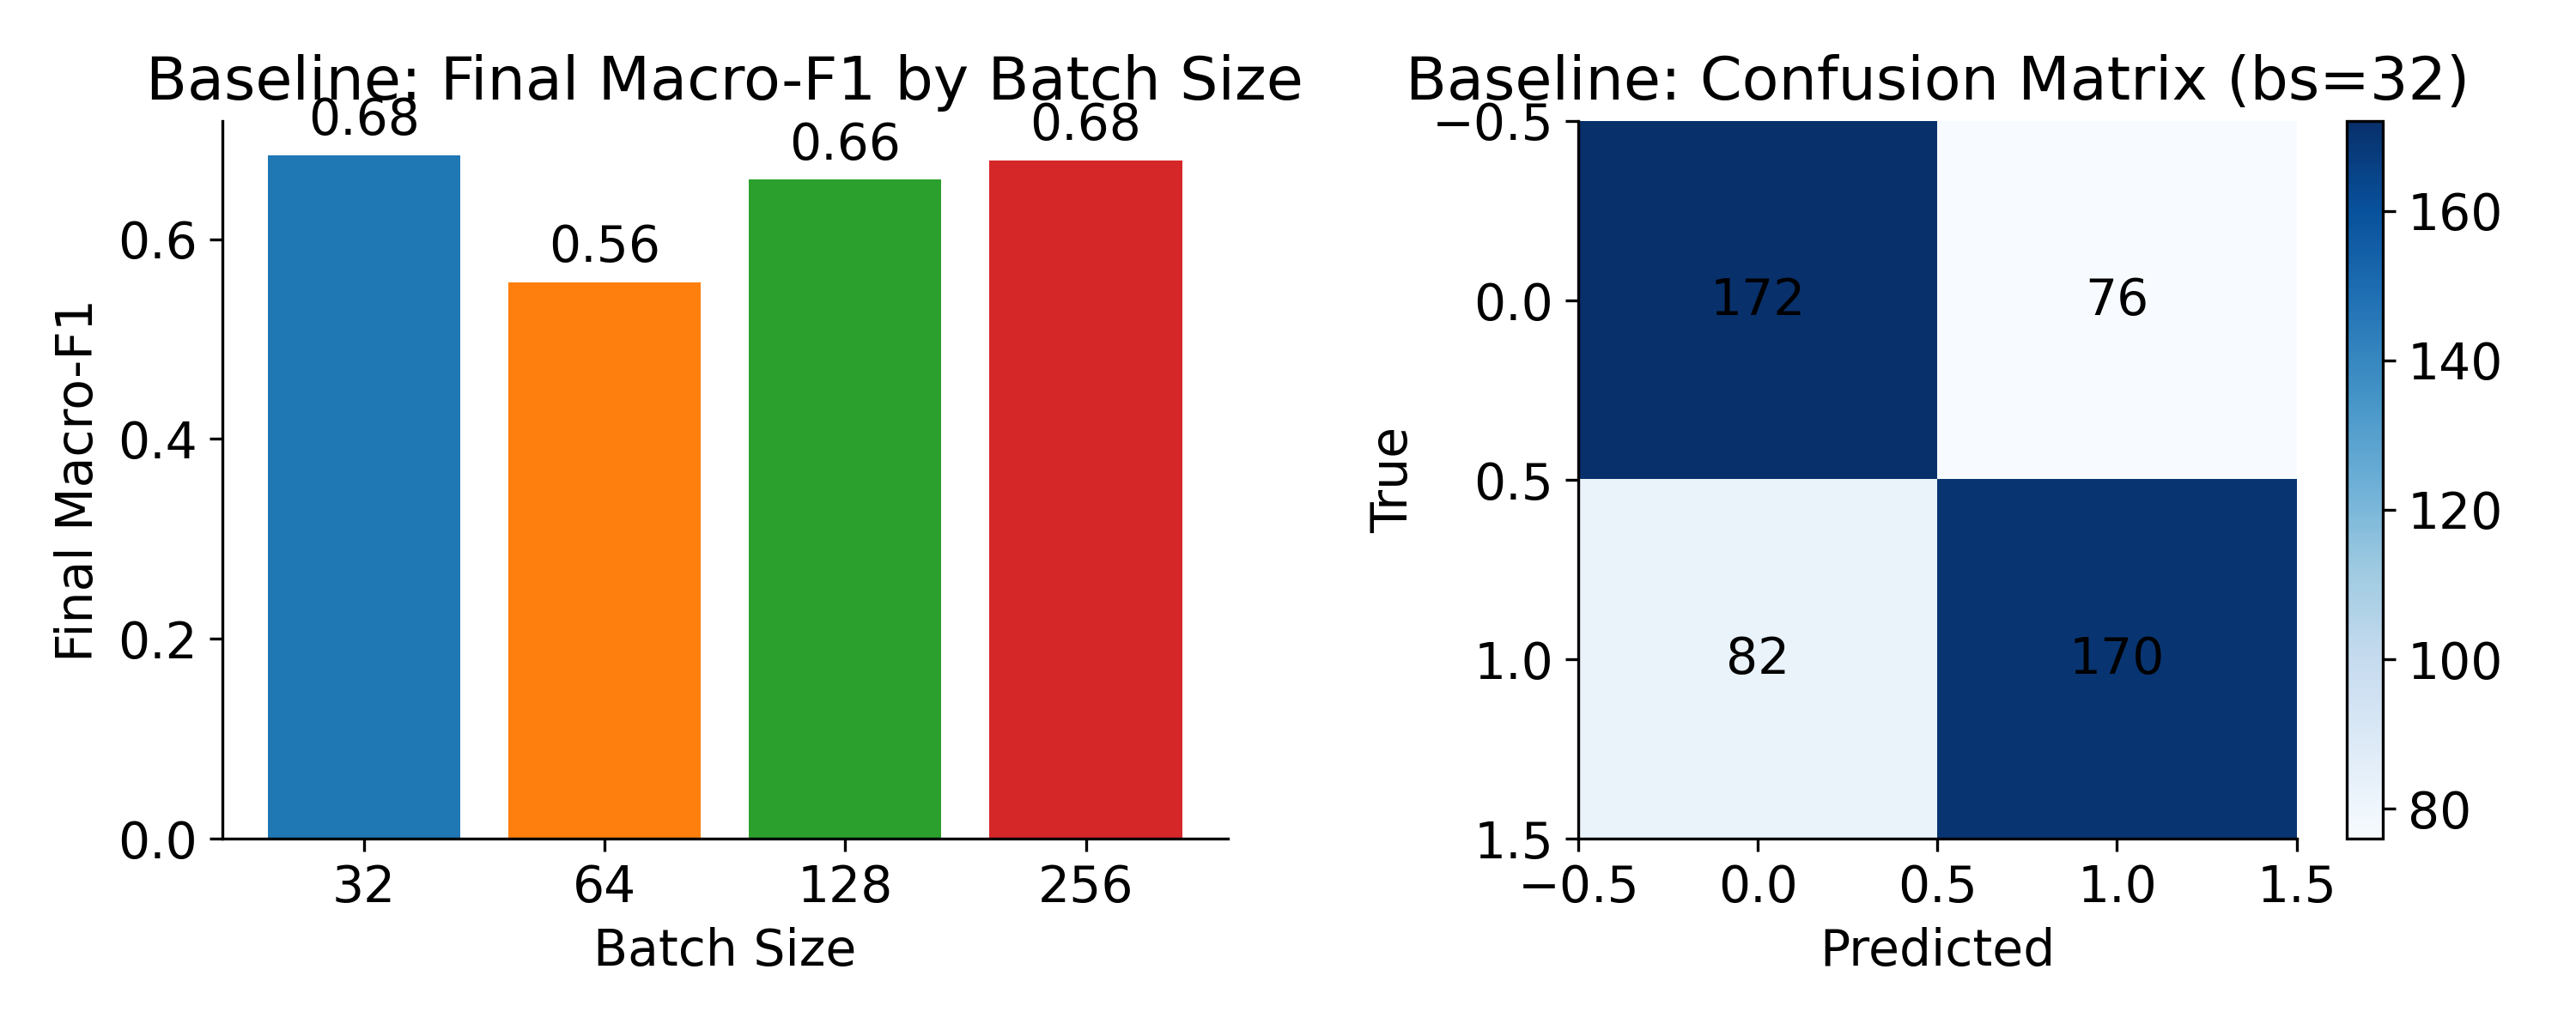
\includegraphics[width=0.45\textwidth]{Baseline_final_f1_and_confusion.png}
\end{center}
Figure\,1 illustrates training instability and confusion matrix outcomes for a GRU-based baseline. 

\begin{center}
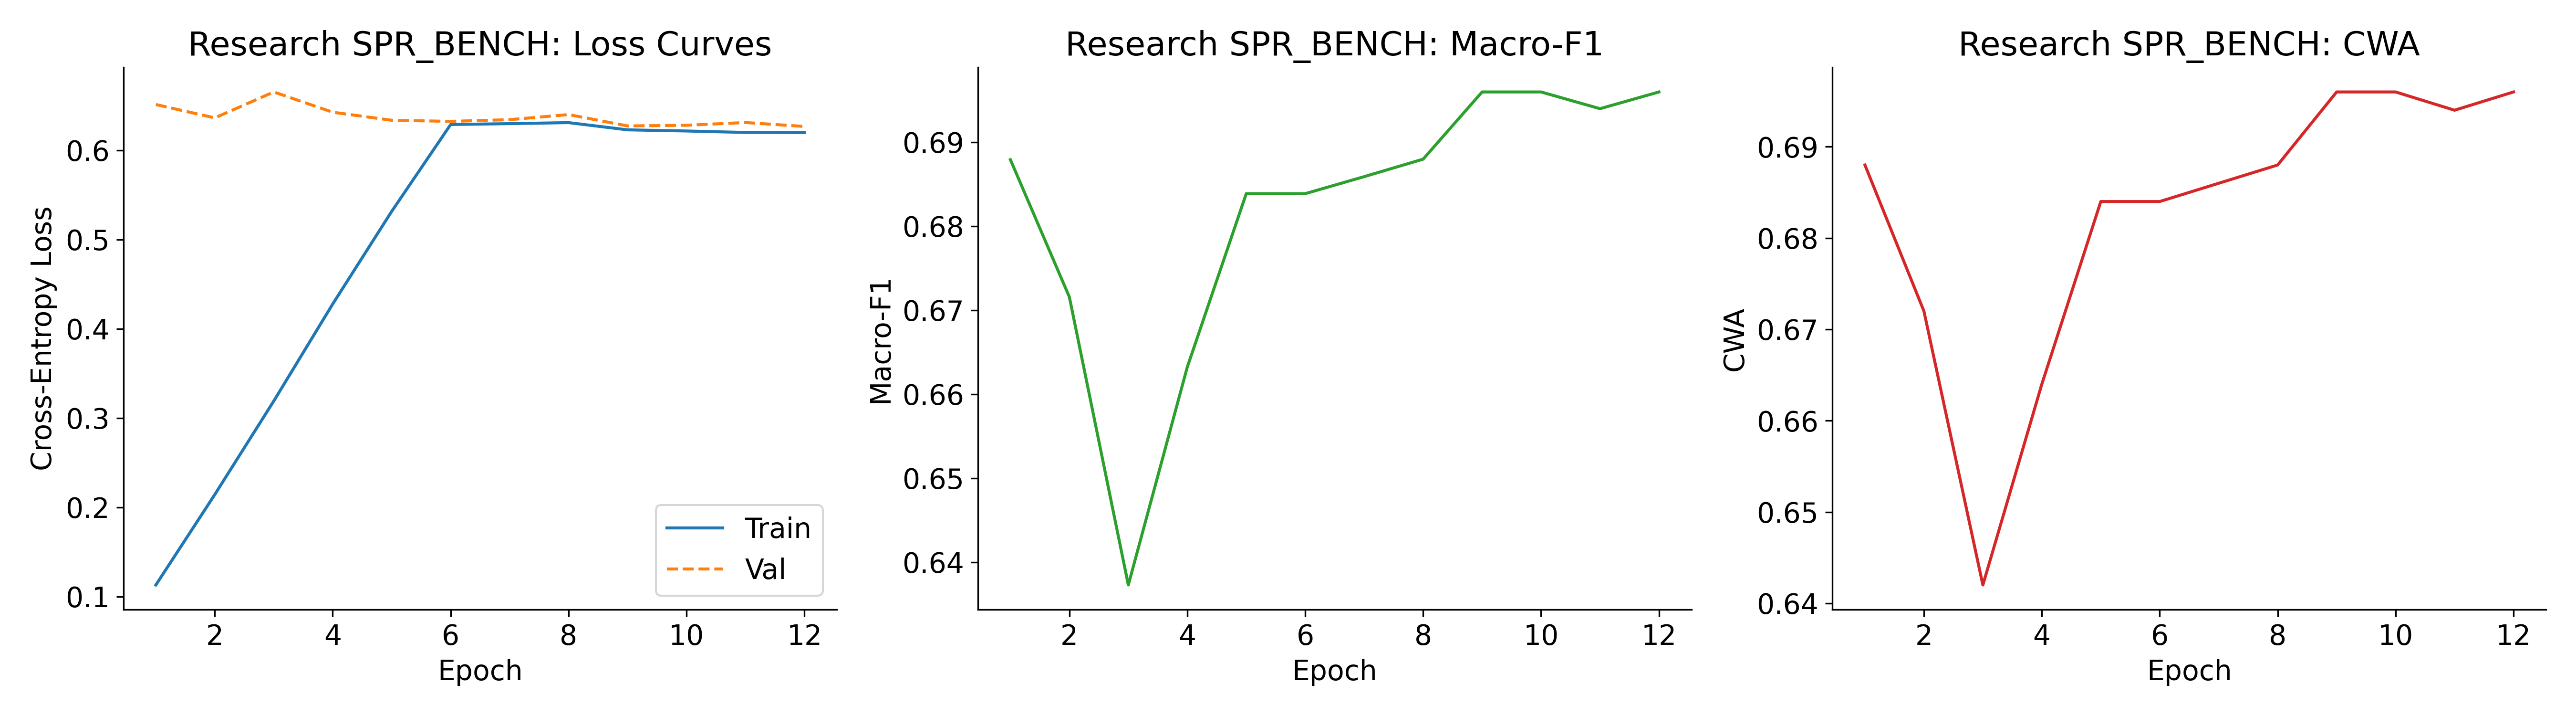
\includegraphics[width=0.45\textwidth]{Research_loss_f1_cwa.png}
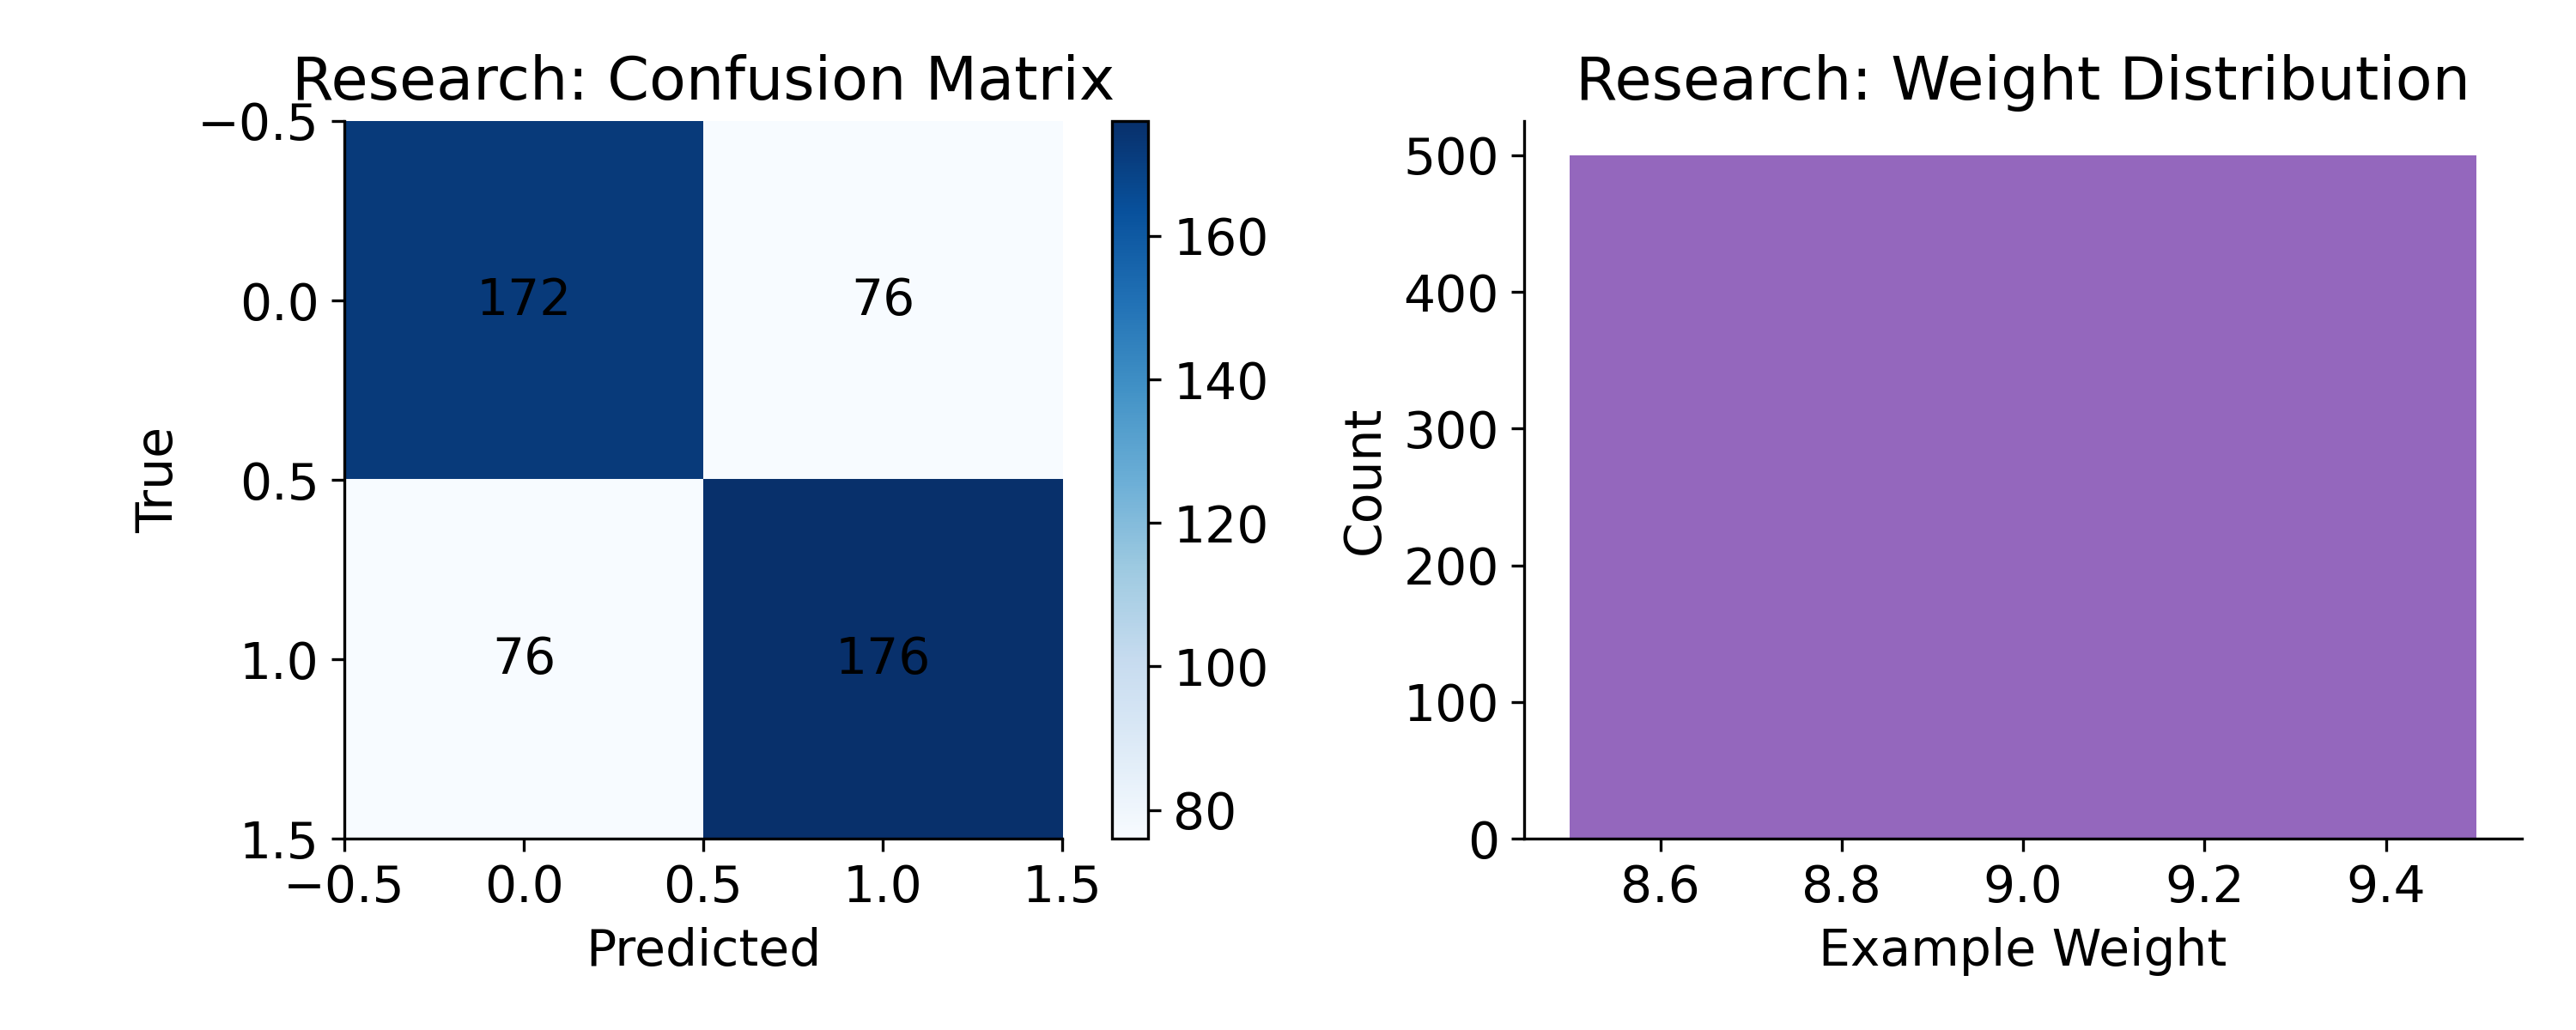
\includegraphics[width=0.45\textwidth]{Research_confusion_weight.png}
\end{center}
Figure\,2 highlights the complexity-weighted accuracy of a Transformer model, showing partial gains yet susceptibility to certain classes.

\section{Conclusion}
We show that standard deep models can exhibit unstable or incomplete solutions to symbolic tasks. Lessons learned indicate that careful data curation, hyperparameter tuning, and interpretability measures are critical. Future work lies in designing robust interventions to handle compositional constraints more reliably.

\bibliographystyle{plain}
\bibliography{references}

\appendix

\section{Additional Experiments}
Further ablation results and training configurations are presented here. We include additional confusion matrices, label distributions, and performance metrics that validate our main claims while illustrating overlooked complexities in symbolic reasoning.

\end{document}